\chapter{Vulnerable Function Call- Tracing Exploratory Study}
\label{sec:exploratory_study}
%\section{Introduction}
\begin{comment}To analyze the impact of safe clients, I explored how clean and used client projects react to vulnerability library updates. 
In order to do that, I performed an exploratory study at the function level and access of the library Application Programming Interface (i.e., API). 
\end{comment}

The objective of the exploratory study is to understand to what extent the usage of the library vulnerable code affects the way developers update their vulnerable dependencies.

\section{Approach}
%%%%%%%%%%%%%%%%%%%%%%%%%%%%%%%%%%%%%
\begin{figure*}[ht]
\centering
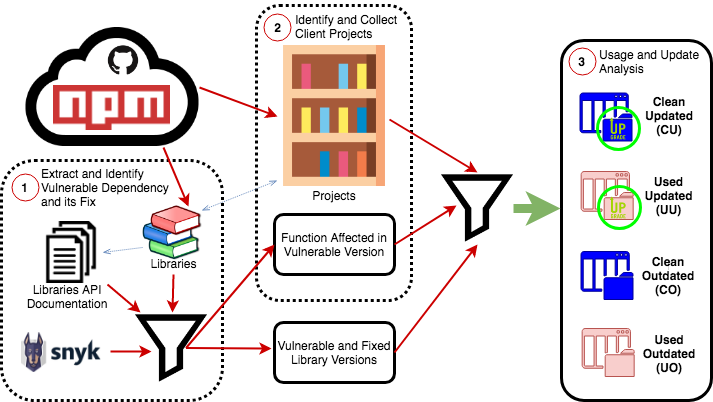
\includegraphics[width=1\textwidth]{images/exploratory_approach.png}
\caption{An Overview of our approach, comprises of three steps (i) Extract and Identify Vulnerable Dependency and its Fix (ii) Identify and Collect Client Projects (iii) Usage and Update Analysis.}
\label{fig:example}
\end{figure*}
%%%%%%%%%%%%%%%%%%%%%%%%%%%%%%%%%%%%%

Figure \ref{fig:example} depicts an overview of our approach, which is detailed in three steps.
I used a manual investigation to validate the mapping of both (i) identification of the vulnerability fix and the affected API and (ii) identification of how the client calls the vulnerable API.
I will now describe each step in detail.
\begin{itemize}
    \item \textbf{Step One: Extract and Identify the Vulnerable Dependency and its Fix} \\
    From the Snyk website\footnote{data was mined from website \url{https://snyk.io/vuln}}, I collected the fix information for the vulnerability issue (i.e., in the form of the pull request (PR), GitHub issue and the commit location). 
    The output is the identification of the code fixes and the affected API that a client project may use.
    
    \item \textbf{Step Two: Identify and Collect Client Projects } \\
    Taking the output from Step One, for Step Two I mined and collected npmJS projects\footnote{data was mined from the npmjs website at \url{https://www.npmjs.com}} from GitHub that used the vulnerable dependency.
    Then I mined the client project repository to identify whether or not the client had migrated to a cleaner version of the dependency.
    This was done by inspecting the \texttt{package.json} meta-file to see whether or not the vulnerable dependency was updated to a newer version.
    Hence, the output is a sample of client projects that have either (i) migrated away from the vulnerable dependency (i.e., Updated) or (ii) are still dependent on the vulnerable dependency (i.e., Outdated). 
    
    \item \textbf{Step Three: Usage and Update Analysis} \\
    Taking the outputs of Step One and Two, for Step Three I classified client projects based on (i) their update status (i.e., Updated or Outdated) and (ii) whether or not they explicitly used the affected vulnerability in their client code.
    As such, the output was a classification of the client projects based on the  following update patterns: 
\begin{enumerate}
    \item \textit{Clean and Updated (CU)}: refers to clients that are using the vulnerable dependency, but were not using the affected function in their projects. These projects are deemed \textit{safely mitigated}, as they have migrated away from the vulnerable version. 
    
    \item \textit{Used and Updated (UU)}: refers to clients that are using both the vulnerable dependency and the affected function in their projects. These projects are deemed \textit{safely mitigated}, as they have migrated away from the vulnerable version. 
    
    \item \textit{Clean and Outdated (CO)}: refers to clients that are using the vulnerable dependency but are not using the affected function in their projects. These projects are deemed \textit{potentially unsafe} as they have not migrated to the safe version.
    
    \item \textit{Used and Outdated (UO)} : refers to clients that are using both the vulnerable dependency and the affected function in their projects. These projects are deemed \textit{unsafe} as an attack is able to compromise the client project.
\end{enumerate}
\end{itemize}

The analysis results will be reported in two sets. In the first set, I will report on the proportion of each update patterns (i.e., CU, UU, CO and UO). My intention is to understand if using the vulnerable function has an impact on whether or not the client project dependency will be updated.

For the second set, I will analyze the time taken to update for projects that followed the CU and UU update patterns. 
My intention is to understand which one of these patterns updates first. 

\section{Case Study Setup}
As shown in the Table \ref{tab:vulnerability}, the three vulnerable dependencies were chosen due to their high severity and their impact (popularity) to the npm ecosystem of packages (i.e., we used the number of GitHub stars and downloads to rank popularity). 

\vspace{3mm}
%%%%%%%%%%%%%%%%%%%%%%%%%%%%%%%%%%
\begin{table*}[ht]
\centering
\hspace*{-2cm}
\scalebox{0.7}{
\begin{tabular}{|l|l|l|l|l|l|l|}
\hline
\multicolumn{1}{|c|}{\textbf{Dependency}} & \multicolumn{1}{c|}{\textbf{Severity}} & \multicolumn{1}{c|}{\textbf{Snyk ID}} & \multicolumn{1}{c|}{\textbf{General Description}} & \multicolumn{1}{c|}{\textbf{Affected versions}} & \multicolumn{1}{c|}{\textbf{Disclosed}} & \multicolumn{1}{c|}{\textbf{Published in Snyk}} \\ \hline
angular & High & npm:angular:20131113 & Protection Bypass & \textless 1.2.2 & 12 Nov 2013 & 23 Jan 2017 \\ \hline
marked & High & npm:marked:20150520 & Content \& Code Injection (XSS) & \textless 0.3.6 & 20 May 2015 & 20 Apr 2016 \\ \hline
ws & High & npm:ws:20160624 & Denial of Service (DoS) & \textless{}= 1.1.0 & 24 Jun 2016 & 26 Jun 2016 \\ \hline
\end{tabular}}
\caption{Summary of the three Selected Vulnerable Dependencies}
\label{tab:vulnerability}
\end{table*}
%%%%%%%%%%%%%%%%%%%%%%%%%%%%%%%%%%

As well as the \texttt{ws} package from the motivating example in chapter \ref{sec:background}, the other two studied vulnerabilities are the popular \texttt{angular} and \texttt{marked} libraries.
It is important to note that I selected security vulnerabilities that were published at least a year ago before this study, allowing ample time for client projects to become aware of the security advisories.

For the client selection, as shown in Table \ref{tab:selected_project}, I selected the top projects based on popularity (i.e., GitHub stars, dependents and download counts).

\vspace{3mm}
%%%%%%%%%%%%%%%%%%%%%%%%%%%%%%%%%%
\begin{table*}[ht]
\centering
\scalebox{0.8}{
\begin{tabular}{|l|r|r|r|r|r|}
\hline
\multicolumn{1}{|c|}{\multirow{2}{*}{\textbf{Dependency}}} & \multicolumn{1}{c|}{\multirow{2}{*}{\textbf{\# GitHub stars}}} & \multicolumn{2}{c|}{\textbf{Updated dependents}} & \multicolumn{2}{c|}{\textbf{Outdated dependents}} \\ \cline{3-6} 
\multicolumn{1}{|c|}{} & \multicolumn{1}{c|}{} & \multicolumn{1}{c|}{\textbf{Max stars}} & \multicolumn{1}{c|}{\textbf{Min stars}} & \multicolumn{1}{c|}{\textbf{Max stars}} & \multicolumn{1}{c|}{\textbf{Min stars}} \\ \hline
angular & 58,610 & 886 & 63 & 390 & 7 \\ \hline
marked & 16,459 & 3,614 & 176 & 11,448 & 1,021 \\ \hline
ws & 8,751 & 15,145 & 691 & 64,907 & 1,092 \\ \hline
\end{tabular}}
\caption{Summary of the 60 Selected Client Popularity (measured by GitHub stars). \textit{Note: 30 clients (Updated) had migrated, while 30 clients (Outdated) still depend on the vulnerable dependency.}}
\label{tab:selected_project}
\end{table*}
%%%%%%%%%%%%%%%%%%%%%%%%%%%%%%%%%%

My assumption is that popular libraries are more likely to be updated.
I sampled 10 updated and 10 outdated client projects for each vulnerability, resulting in 60 client projects for the case study.

%%%%%%%%%%%%%%%%%%%%%%%%%%%%%%%%%%%%%
\begin{figure}[ht]
\centering
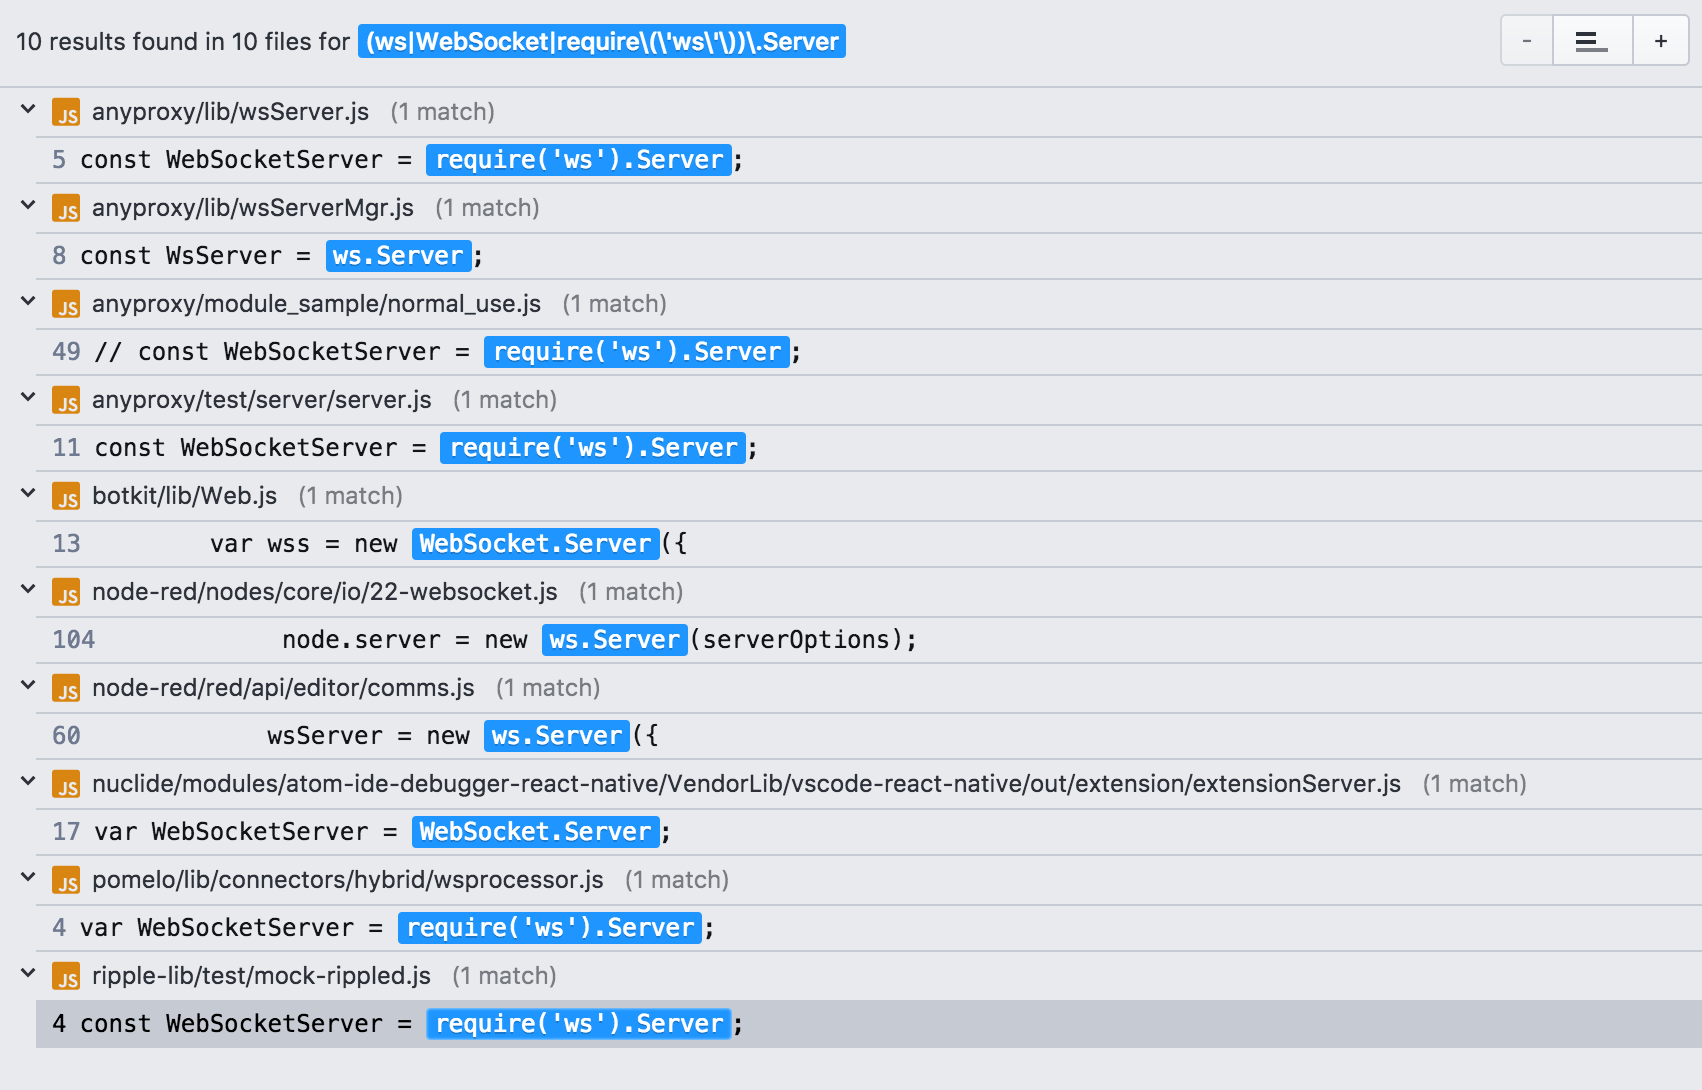
\includegraphics[trim={0 0 0 2.5cm},width=1\textwidth]{images/UU_ws.png}
\caption{Example of the regular expression used and the results showing the possible locations provided by the text editor tool}
\label{fig:regExp}
\end{figure}
%%%%%%%%%%%%%%%%%%%%%%%%%%%%%%%%%%%%%

I manually investigated each vulnerability and usage within the client.
In step one, I examined the git commit history to manually trace the change commit of the vulnerability to an API.
For step two, I downloaded the git repository for each project and checkout the corresponding commit, afterwards as shown in figure \ref{fig:regExp} with the help of a simple regular expression search\footnote{for the search I used the atom text editor to load the vulnerable version of the client and executed the search}, using the keywords described in table \ref{tab:keywords} I located possible locations where the client would be using the library API. 
Then I manually validated that the client was using the library API.

%%%%%%%%%%%%%%%%%%%%%%%%%%%%%%%%%%
\begin{table*}[ht]
\centering
\hspace*{-0.3cm}
\scalebox{0.75}{
\begin{tabular}{|l|l|l|l|l|l|l|}
\hline
\multicolumn{1}{|c|}{\textbf{Dependency}} & 
\multicolumn{1}{c|}{\textbf{Fixed function}} & 
\multicolumn{1}{c|}{\textbf{Mapped APIs}} & 
\multicolumn{1}{c|}{\textbf{Keywords used in searching client code}} \\ \hline
angular &getTrustedContext&\$compileProvider&\$compileProvider \\ \hline
marked &unescape& Renderer, InlineLexer&.Renderer, InlineLexer \\ \hline
ws &websocketserver&websocket.server& ws, WebSocket, require('ws').Server, .Server \\ \hline
\end{tabular}}
\caption{Summary of the Keywords Used in the Validation Mapping}
\label{tab:keywords}
\end{table*}
%%%%%%%%%%%%%%%%%%%%%%%%%%%%%%%%%%

\section{Results and Implications}
The results will be presented in two sets.

(First Set): \textbf{73.3\% (22 out of 30) outdated clients do not use the vulnerable code.} 
Figure \ref{fig:results1} shows the results of the first set.
Interestingly, while analyzing two out of the three libraries, I found that even if the client projects were using the vulnerable library most of them were not executing the affected function (UO).

%%%%%%%%%%%%%%%%%%%%%%%%%%%%%%%%%%%%%
\begin{figure}[ht]
\centering
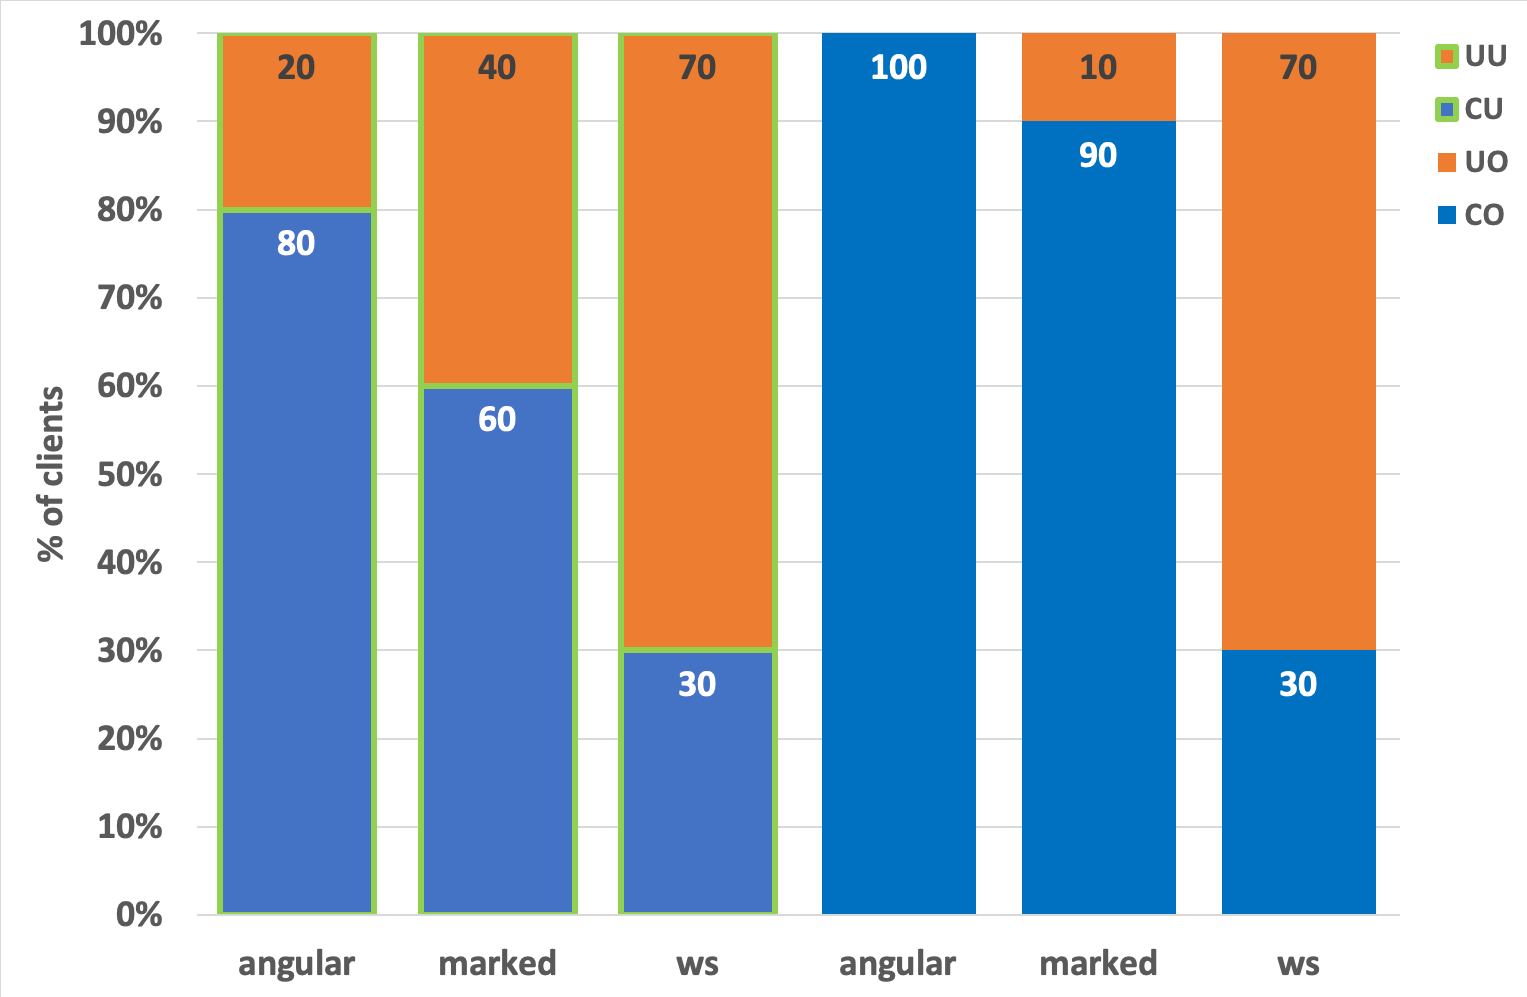
\includegraphics[width=1\textwidth]{images/exploratory_results.png}
\caption{Proportion of each update pattern for the 30 Updated (CU, UU) and 30 Outdated (CO, UO) client projects.}
\label{fig:results1}
\end{figure}
%%%%%%%%%%%%%%%%%%%%%%%%%%%%%%%%%%%%%

On the contrary, I found especially in \texttt{angular} and \texttt{marked} client projects, that a high proportion of clients that had not migrated away from the vulnerability were indeed clean of the vulnerable code. 
Figure \ref{fig:results1} shows the results of how the \texttt{ws} affecting vulnerability differs from the other two vulnerabilities.
My potential explanation is that the update caused a breaking change, and thus, I speculate that this would require additional migration effort.

(Second Set): \textbf{Clients that do not use the affected function code show a longer delay to migrate away from the vulnerable dependency.} 
Figure \ref{fig:results2} shows, except for the clients of \texttt{ws} project, that clean updated projects (CU) had a wider spread of time taken to update. Similar to the first step, the time taken to fix the \texttt{ws} vulnerability may be related to the fact that it is a breaking change. I speculate that since the client code is not affected by the vulnerability, the developers may either be interested in keeping up to date (i.e., update as soon as possible as the migration effort will be low) or satisfied with the current state (i.e., if it is not broken, it is better not to fix).

%%%%%%%%%%%%%%%%%%%%%%%%%%%%%%%%%%%%%
\begin{figure}[ht]
\centering
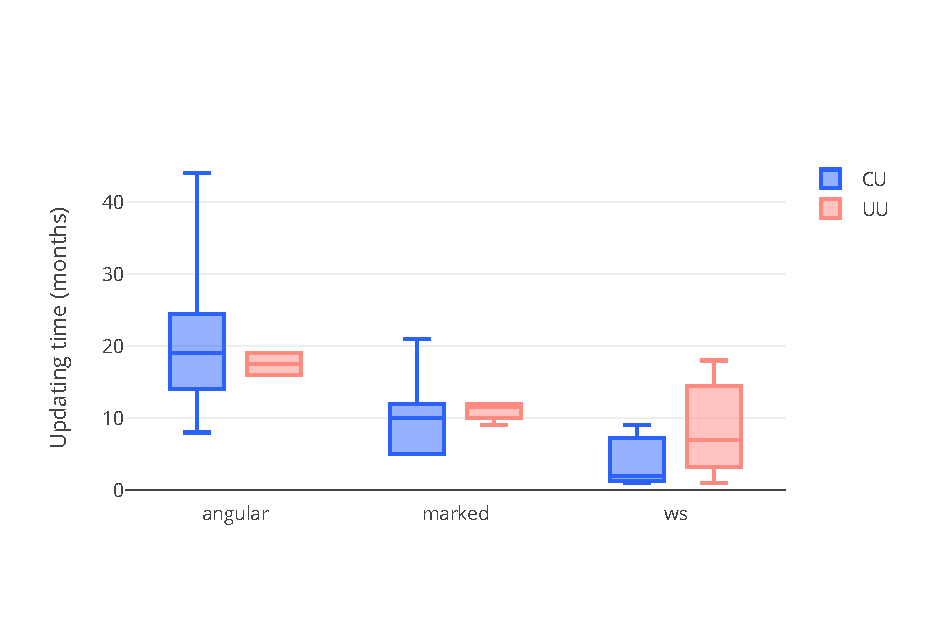
\includegraphics[width=1\textwidth]{images/box.pdf}
\caption{Time taken (months) for the updated clients (CU, UU) to migrate away from the vulnerable dependency.}
\label{fig:results2}
\end{figure}
%%%%%%%%%%%%%%%%%%%%%%%%%%%%%%%%%%%%%

After analyzing the previous results I came with the following implications:
\begin{enumerate}
    \item \textit{Security vulnerability analysis at the dependency level is likely to be an overestimation.}
    The results of the study provide evidence that many of the outdated project are free of the vulnerability.
    This insight is an indication that more analysis at the function level is needed to support this claim.

    \item \textit{Automatic approaches are needed to increase the scalability of mapping the usage of library code in client projects. }
    A potential avenue for future work is the automation of my current approach.
    Currently, my projects are a limited sample of the population. 
    With automation, the same study can be conducted at a larger scale providing a more accurate comprehensive analysis.
\end{enumerate}